% Chapter Template

\chapter{Implementation 10} % Main chapter title
%Possible solutions (in the context)
\label{Chapter4} % For referencing the chapter elsewhere, use \ref{Chapter1} 

After introducing the project, we will now talk about our implementation.
Our implementation used the aforementioned tools as well as some smaller libaries that will be explained in the following section.
\section{Architecture}
We tried to integrate a SoA, so that our components would be self-contained and reusable. 
For example, the communication to Unity should still work if a connection to the webserver failed.

The Tcp and Serial connection whre set-up in a general way (send/receive all). 

As a consequence, the processing of the data would happen in another component.

The front-end connection received it's own namespace for socket.io events so front-end relevant data 
would only be proccessed in it's set namespace component.
%picture of our architecture
\section{Prototyping}
Our reasearch inspired us to try Rapid Prototyping in our project. 
We designed a Proof of Concept for each stage of our implementation (\ref{fig:PoC}).
\begin{figure}[th]
	\centering
	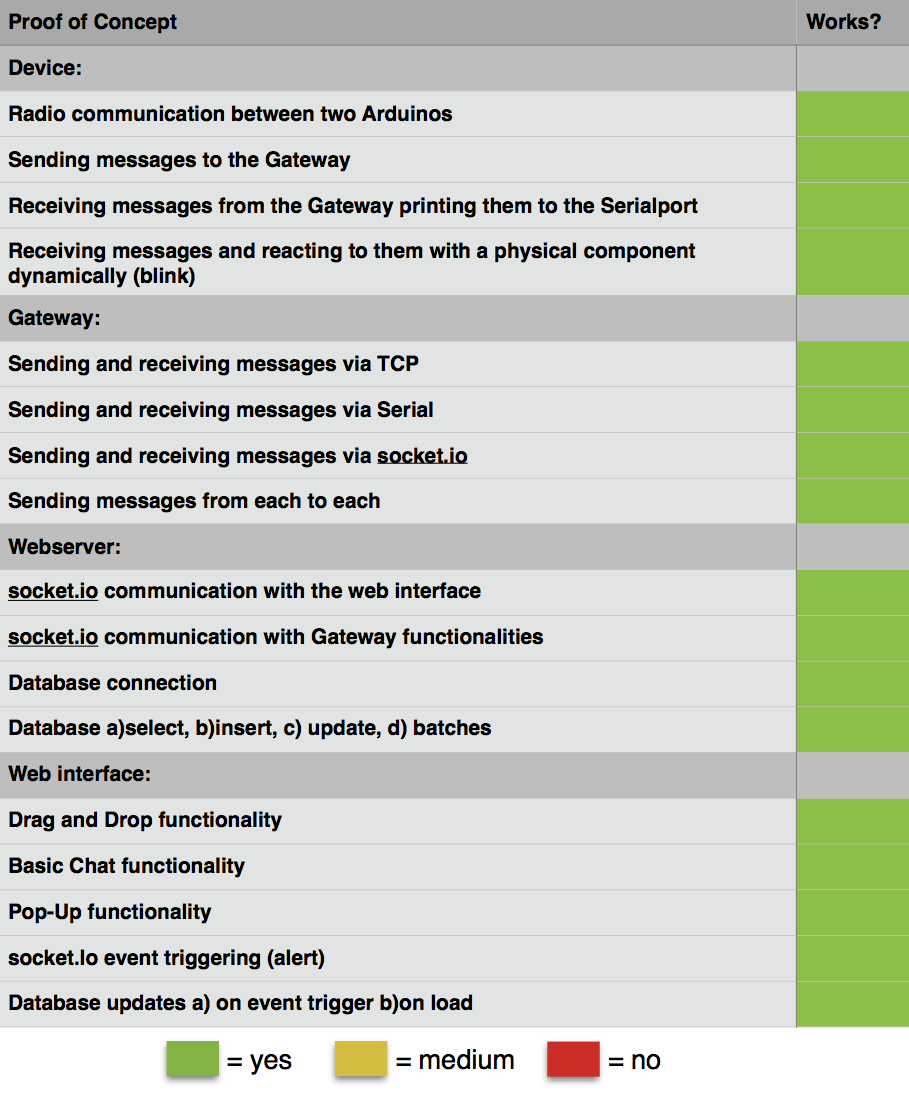
\includegraphics[width=100mm,scale=1]{Figures/PoC}
	\decoRule
	\caption[PoC]{List of our PoC steps}
	\label{fig:PoC}
\end{figure}

Our final result is a MVP %Reference abkürzung 
which provides the bare functionalites but lacks in design and more extensive features which we will eleborate in the evaluation.
\section{Device}
Since the room consisted of microcontroller-driven-riddles only at the time of this thesis, we decided to design a prototype and a template for integration of future microcontroller-driven-riddles.
%Fig: Arduino verkabelung für prototype

The template was designed to simplify the process of developing a riddle.
The escape room provided in it's prior form no support for new riddle-developers. 
We decided to modify the existing communication protocol, but had to be careful not to impact communication to the existing riddles.

Still, we wanted simplify the communication system for riddle-developers. 

The existing communcation protocol followed a "string-to-chararray-send" and "receive-chararray-to-string" structure that we applied to our implementation.
In contrast to the existing puzzles though, we decided to separate the code into several parts, named by the functionality they supplied. 

 %Chararrays are smaller than strings hence faster for radio-communication.
The template is devided into 3 parts: "Groundwork", "Riddlefunctionality" and "Remote Functionality". 

The "Groundwork" section should be filled with libaries, variables and definitions. 

The "Riddlefunctionality" section should contain the riddles functionalities seperated from nearly any communication. 
The only communication that needs to be defined there is when the Microcontroller should send messages and which. That is executed by writing a single line command containing the desired string.
If the string's value is defined in the "registerRiddle()" function of the "Remote Functionality" section, it will be translated in the web interface. 

Likewise should the "Remote Functionality" section contain any remote commands for interaction with the web interface and the server.
The "Remote Functionality" section consists of two functions: 

"registerRiddle()" where strings to be send once on starting the device are defined. 
These strings set the configuration of the variables in the web interface.
To work, they need to follow a specific structure:
\begin{enumerate}
    \item an Index for the riddlevariable (to order the variables)
    \item a "readonly" or "write" command (to make it static or dynamic)
    \item the name of the variable (to translate)
    \item the value of the variable (needs to be converted into a String)
    \item an optional button value (if it was present, a button would show)
\end{enumerate}
That structure is meant to be applieable for any variable. 

\begin{figure}[th]
	\centering
	\includegraphics[width=75mm,scale=0.75]{Figures/registerRiddle}
	\decoRule
	\caption[FrontViewTable]{"registerRiddle" definition in the Arduino IDE}
	\label{fig:FrontViewTable}
\end{figure}


The other function is named "remoteCommand()" and designed to contain processing of incoming messages from the gateway/Pc.
It's connected to the radio functionality further down in the code, nevertheless allows the user not to care about how the messages are processed.

The developer is advised to use a "Switch-Case" structure to define the microcontroller's reactions to radio messages, to keep the processing clean and standartized. 
For any reaction concerning the defined variables, the case should match the index of the variable in order for the buttons within the web interface to work.
%fig arduino def

The documentation we provided explains the template in further detail.

For our prototype, we used an Arduino Uno with a RFM69HCW module, a keypad, and an I2C-display. 
The riddle would be to guess a code and enter it. 
We wanted the code to be changeable to provide different difficulties. 
Moreover would the riddle possess static  "won", "lost", and "reset"-values to track and control the riddle's state.
%prototype pic
\section{Back-End}
We used the relational model to manage our database. 
In the relational model, related records are linked by a key predicate common to all. 
In our project, we found that two tables fit our needs. 
One table manages the location, name and other general information about the riddle displayed in the main view, 
whereas the other one is responsible for saving and editing the information displayed in the pop-up window. 
This seperation simplifies database changes, clearifying the tasks happening on the Node.js server.
The Node.js server connects the information when sending to the front-end by assigning the details with the riddle's id to the corresponding riddle. 

\section{Middleware}

\subsection{Web Server}
It quickly became apperant that our middleware web server would use Node.js due to the reasons mentioned above.
The decisive factor for this decision was that it would be easier to develop and understand a web server programmed in the same language as the front-end.

As we did all website operations client-side, Node.js main operation was the database and handling. 
We used the "pg-promise" libary \parencite{pg-promise} for our database integration with postgres. 

Depending on the event emittet by the web interface, database-queries to select, update or delete entries could be triggered.

If the gateway emittet a message, a control mechanism would check if the riddle was known and either add a new riddle, update an existing riddle (if new variables where recognized) or translate the incoming data .

With Socket.io, the client would register whether a front-end or another client would register and forward the needed data from the database. 
By namespacing (creating different channels for different clients), we tried to avoid dispensable traffic.
The gateway would receive the changeable ("write") values and send them to the connected riddles.
The front-end would receive the sorted database data in a sorted json fit to the front-ends data-handling.

%Architecture We tried to implement our functionalities as loosely as possibilities, so 
\subsection{TCP/Serial/Socket.IO-Client}
This part of the middleware changed several times during our developing process. 
Since the front-end allowed a reassignement of the messages that would trigger an Unityevent, a middleware implementation was needed.
We decided to filter the relevant "Finish"-serialmessages through a PostgreSQL-database, which is compatible with different languages and frameworks.
Additionaly, we needed to implement a connection from the serial port to our socket.io connection.

First, we wanted to use the existing C++-server for our architecture but discovered quickly that understanding and extending the existing code would probably take longer than recreating the features.

Then, because many developers of our target group were proficient in C\# from Unity development, we tried to implement the functionalites with a .NET WPF-App.
This proved to be difficult, as it required multi-threading and communication between the threads. Both are well documented at the MSDN \parencite{MSDN}, 
however due to the mass of different techniques it was hard to get an overview. 
The code we created was easier than the C++ code, though not comparable to the readability of the Javascript-code.
It took us roughly a week to implement the desired functionalites. 

Finally, we decided to revisit our C\# code and tried to implement it in Javascript.
The same functionalites took us about 6 hours to implement, though we did by then have intermediate experience in Javascript and started our C\# implementation with Unity-C\#-Knowledge.
In our perception, the async-capabilities of Node.js showed a tremendous advantage compared to the threading difficulties wie experienced with the .NET project.

\begin{figure}[th]
	\centering
	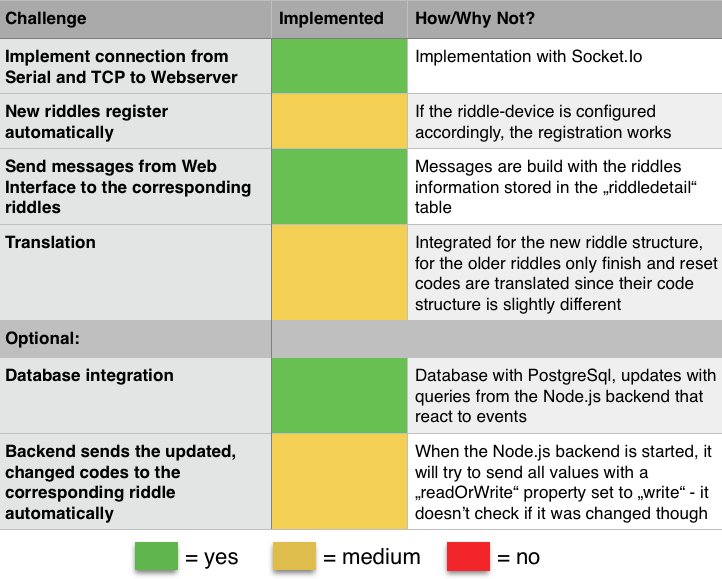
\includegraphics[width=75mm,scale=0.75]{Figures/backendOverview}
	\decoRule
	\caption[FrontViewTable]{Overview about our front-view challenges.}
	\label{fig:FrontViewTable}
\end{figure}

\section{Front-End}
For setting up our front-end, we used the Create-React-App which provides a front-end build pipeline with Babel and Webpack.
React recommends to start there for single-page applications \parencite{createReactApp}. 

It provides a package.json file where  which version of a module one wants to use is defined. 
This prevents unwanted updates so the existing code won't risk becoming deprecated.

The npm installer (which is the standard installer for React and Node.js) automatically generates a package-lock.json file which saves the dependency tree in further detail.
We discovered GIT-difficulties with the modules and were thankful that we could reinstall the needed packages without having to search which modules we needed.

For our file-structure, we used the recommended approach to group by filetype \parencite{reactStructure} in combination with the Create-React-App-structure.
%Fig: Our File structure front end

Starting out, we wanted to implement a node-editor to connect riddles in all thinkable ways. 
When we listed our wished functionalities (Changeable riddleassignments with "Single", "AND" and "OR" connections to the Unity-Events) we decided that a drag-and-drop table would supply those functionalites (Changeable assignements, OR connections) without creating a difficult User-Interface.
We used the React-dnd libary \parencite{reactDND} to implement the drag-and-drop functionality in React. Currently, it works only on PC since we thought that would be a more popular use case, but adding a mobile implementation for the module is possible.

When a user dropped a riddle into a "Video" field (and saved), the riddle's "Finish"-command would be reassigned on input to the corresponding Video-Trigger-command. 
For example, the "Video1" command was originally triggered by "Riddle1". 
If a user wanted to make "Riddle2" trigger "Video1", he needed to replace "Riddle1" in the "Video1"-List with "Riddle2". 
Whenever "Riddle2" would now signal it's finished, the "Finish"-code of "Riddle1" would be sent to Unity via TCP.

If a Riddle was newly registered, it would be named "NewRiddle" and appear in the "Unassigned Riddles"-List on the web interface.
We designed an "Edit"-function which enabled changing the name of the riddle and deleting it in case it got corrupted (or deleted in real-life).

Another aspect was the popup-window for the riddles. We wanted it to show enough information, yet keep it simple. 
Consequently, our layout for the popup-window was designed flexibly to adapt to a desirable output depending on the usecase:

Each variable would be displayed in respect to it's in the Arduino defined values. 
If a variable was set "readonly", but didn't have a button value defined, the information would be listed plainly.
If a variable was set "write", but didn't have a button value defined, the information would be listed plainly. 
Additionaly, an input field would enable changing the defined value and sending it to the Arduino automatically next time the Server would start. 

If the microcontroller was programmed to interpret the incoming value, a variable could be changed that way (e.g. a password in a riddle).
If a button component was set in a variable, a button would appear instead of plain information about the variable. 
The user would be able to click the button to send the code immediately to the riddle. 
This functionality was especially designed with "Finish" and "Start" functionalities in mind, where a supervisor of the escape room might want to trigger these functionalites during a game if customers get stuck.

To increase the general overview for a supervisor, the color of a riddle would change to green once it's "Finish"-code arrived.

\begin{figure}[th]
	\centering
	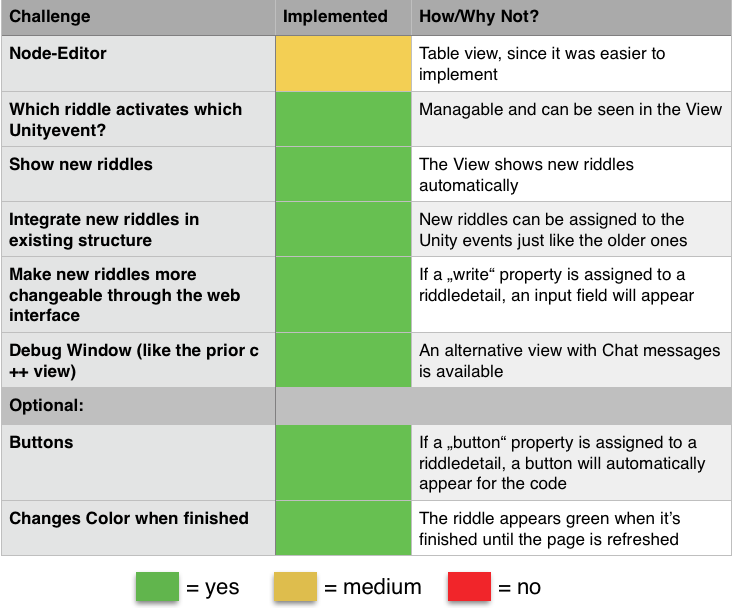
\includegraphics[width=75mm,scale=0.75]{Figures/frontendOverview}
	\decoRule
	\caption[FrontViewTable]{Overview about our front-view tasks.}
	\label{fig:FrontViewTable}
\end{figure}



